\renewcommand{\code}[1]{\mintinline{elixir}{#1}}
\subsection{A Pinch of Formalization}

\begin{frame}[fragile]
\frametitle{A Pinch of Formalization}\transdissolve
\color{darkslateblue}
\begin{minipage}{\textwidth}
\color<2->{gray}
  \begin{figure}
  \centering
  $\alpha$ type variables, $c$ constants, $x$ variables
  \begin{grammarfig}
    \text{Base types}  & b &\bnfeq& \intTop \bnfor \atomTop \bnfor \texttt{function} \bnfor \texttt{tuple} \\[1mm]
    \text{Types}       & t,s &\bnfeq& b \bnfor c  \bnfor \alpha \bnfor \fun{\ov{t}}{t}
    \bnfor  \tuple{\,\ov{t}\,} \color<2->{magenta}\bnfor t \lor t  \bnfor t\land t \bnfor \neg t\\[2mm]
    \text{Expressions} & e, f &\bnfeq& c\bnfor x\bnfor  \textcolor<2->{typeBlue}{\lam{\ov{x}}{e}}
    \bnfor\app{f}{\ov{e}}\bnfor\tuple{\,\ov{e}\,} \bnfor \elem{e}{e} \\[1.5mm]
    &&\bnfor& \tlet{x}{t}{e}{e}
    \bnfor \color<2->{typeBlue} \caseExpr{} \\[2mm]
\color<3>{newgreen}    \text{Patterns}
\color<3>{newgreen}    &p &\bnfeq& \color<3>{newgreen}x \bnfor c \bnfor \tuple{\,\ov{p}\,} \\[1mm]
\color<3>{newgreen}    \text{Guards}
\color<3>{newgreen}    &g &\bnfeq&\color<3>{newgreen} \gand{g}{g} \bnfor \gor{g}{g} \bnfor \gnot{g} \bnfor \isInt{d}  \\
\color<3>{newgreen}    &&\bnfor&\color<3>{newgreen} \isAtom{d} \bnfor \isTuple{d} \bnfor \isFunction{d}{d}  \\
\color<3>{newgreen}    &&\bnfor&\color<3>{newgreen} \GuardEqq{d}{d} \bnfor \GuardNeq{d}{d} \bnfor \ltt{d}{d} \bnfor \lteq{d}{d}\\[1mm]
 \color<3>{newgreen}   \text{Selectors}
    &d &\bnfeq&\color<3>{newgreen} c\bnfor x\bnfor \elem{d}{d} \bnfor \tupleSize{d}
  \end{grammarfig}
\small\textcolor{gray}{Notation: $\ov{u}= u_1,\ldots,u_n$\quad and we may write \textcolor{darkgray}{$p \;\texttt{when}\; g$} for \textcolor{darkgray}{$pg$}}  
  %  \caption{Expressions and Types}
  \label{fig:types}
\end{figure}
\end{minipage}

\end{frame}


% \begin{frame}
% \frametitle{Types and subtyping}
% \structure{Types as sets of values}

% \begin{center}
%   \hfill
%   $\sem{\texttt{bool}} =\{$\code{true},\,\code{false}$\}$
%   \hfill
%   $\sem{\intTop} = \{$\code{0, 1, -1, 2, -2,} \ldots{}$\}$\hfill\mbox{}\\

%   \bigskip
%   \hfill
%   $\sem{t_1\vee t_2} = \sem{t_1}\cup\sem{t_2}$\hfill
%   $\sem{t_1\wedge t_2} = \sem{t_1}\cap\sem{t_2}$\hfill
%   $\sem{\neg t} = \textsf{Values}\setminus\sem{t}$\hfill\mbox{}
    
% \end{center}


% \bigskip

% \bigskip

% \structure{Subtyping as set containment}


% \[ t_1\leq t_2\quad\iffdef\quad\sem{t_1}\subseteq\sem{t_2}\]

% \end{frame}


\begin{frame}[fragile]\transdissolve
\frametitle{Types for patterns and guards}

\color{black}

\textbf{\large\color{darkslateblue}With guards we lose the property that the set of accepted values is a type}
\medskip
\pause

We can associate to a pair pattern-guard  \textcolor{darkred}{$p$\,\code{when}\,$g$}  two
types (i.e., two sets of values):


\mbox{\textcolor{darkred}{\it Surely accepted type}: largest type containing only
values that match \textcolor{darkred}{$p$\;\code{when}\,$g$} (noted \textcolor{darkred}{$\sAccType{pg}$}) }


\mbox{\textcolor{darkred}{\it Possibly accepted type}: smallest type containing all
values that match \textcolor{darkred}{$p$\,\code{when}\,$g$} (noted \textcolor{darkred}{$\pAccType{pg}$})}


\pause

\begin{block}{Example}
   Let\quad  \textcolor{darkred}{$p$\;\code{when}\,$g$}\quad be  \quad\color{typeGreen}\code{x when (is_map(x) and map_size(x) == 2) or is_list(x)}
  \begin{itemize}
    \item[-] \textcolor{darkred}{$\pAccType{pg}$} = {\color{typeGreen}\code{map() or list()}} \hfill(it
      can accept \alert<4>{only} maps or lists)\vspace{-2mm}
    \item[-] \textcolor{darkred}{$\sAccType{pg}$} =
      {\color{typeGreen}\code{list()}} \hfill(it will \alert<4>{surely} accept all
      the lists)
\end{itemize}
\end{block}

\pause\pause

\textbf{Properties}

\(\left.\begin{array}{lr}
\color<6>{lightgray}- \vdash v:\textcolor<6>{commentgreen}{\sAccType{pg}}\ ~\Rightarrow~\ v \text{ matches }pg
& \text{\color<6>{commentgreen}\color<-5>{white}under}\\
\color<6>{lightgray}- \vdash v:\textcolor<6>{frenchplum}{\pAccType{pg}}\ ~\Leftarrow~\ v \text{ matches }pg
\qquad &\text{\color<6>{frenchplum}\color<-5>{white}over}
\end{array}\pause\right\}\text{-approximate the
  set }\mbox{\color{newgreen}$\{v \mid v \text{ matches }pg\}$}\) 


\end{frame}

\color{black}


% \begin{frame}[fragile]
% \frametitle{Example: Map Size Condition}
% \begin{block}{Function with a map size constraint}
% \begin{minted}[escapeinside=||]{elixir}
% def foo(x) when map_size(x) == 2, do: Map.to_list(x) |\label{foo}|
% \end{minted}
% \end{block}
% \end{frame}

% possibly skippable (uncommon)
% \begin{frame}
% \begin{block}{}
% \begin{minted}[escapeinside=||,fontsize=\scriptsize]{elixir}
% def bar(x) when (is_map(x) and map_size(x) == 2) or is_list(x), do: to_string(x)  |\label{bar}|
% def bar(x) when length(x) == 2, do: x
% \end{minted}
% \end{block}
% \begin{block}{}
% \begin{minted}[escapeinside=!!]{elixir}
% def baz(x, y) when elem(x, 0) == y or is_integer(y) do
%     42
% end
% \end{minted}
% \end{block}
% \end{frame}

% maps
% find examples of debugging thanks to maps
% removed: presentation too long

\begin{frame}[fragile]
\frametitle{Typing pattern matching}

\transdissolve<4->\vspace{.7pt}

\textcolor{darkslateblue}{We use possible/surely accepted types to type case expressions:}

\medskip

Consider \textcolor{typeBlue}{$\case{e}{p_1g_1\to e_1}{....;p_ng_n\to e_n}$} with \textcolor{typeBlue}{$e:t_0$}

\medskip
\pause
the type \textcolor{typeBlue}{$t_i$} of all values that \emph{may} be captured by the
$i$-th branch is

\centerline{\textcolor{typeBlue}{$t_i=(\alert<4>{t_0}\alert<5>{\setminus\bigvee_{j<i}\sAccType{p_jg_j}})\alert<6>{\wedge\pAccType{p_ig_i}}$}}

\medskip

\bigskip
\pause
\textcolor{darkslateblue}{In words:}
the expression \textcolor{typeBlue}{$e_i$} will process  values:

\pause
- generated by \textcolor{typeBlue}{$e$} (i.e., in $t_0$)

\pause

- \alert{minus} those \emph{surely} captured by the previous branches (i.e., in $\bigvee_{j<i}\sAccType{p_jg_j}$)

\pause
- \alert{and} that \emph{may}  match \textcolor{typeBlue}{$p_i$\,\code{when}\,$g_i$} (i.e.,
in ($\pAccType{p_ig_i}$)


\bigskip

\pause

\only<-11>{\[\typingruleExtra{\text{(case)}}
    {\Gamma \vd e : t_0
      \qquad
      ({\footnotesize\forall i<n} \quad \Gamma, \typEnv{t_i}{p_i} \vd e_i : s_i)}
    {\ensuremath{\Gamma \vd \caseExprI{} : \bigvee_{\{i\mid t_i\not\simeq\bott\}} s_i}}
    {\ensuremath{\!\quad t_0\!\!\leq \biglor_{i\leq n} \pAccType{p_ig_i}{}}}
\]
}
\only<12->{\[\typingruleExtra{\text{(case)}}
    {\Gamma \vd e : t_0
      \qquad
      ({\footnotesize\forall i<n} \quad \Gamma, \typEnv{\color{red}t_{ij}}{p_i} \vd e_i : {\color{red}s_{ij}})}
    {\ensuremath{\Gamma \vd \caseExprI{} : \bigvee_{\{i\mid t_i\not\simeq\bott\}} \color{red}s_{ij}}}
    {\ensuremath{\!\quad t_0\!\!\leq \biglor_{i\leq n} \pAccType{p_ig_i}{}}}
\]
\begin{textblock}{5}(13.5,12.5) \footnotesize{\color{red}$(t_i = \bigvee_j t_{ij})$}\end{textblock}
} 
% \only<8>{\begin{textblock}{5}(0,0)
% \includegraphics[scale=1]{images/typecase 1.pdf}
% \end{textblock}}
% \only<9>{\begin{textblock}{5}(0,0)
% \includegraphics[scale=1]{images/typecase 2.pdf}
% \end{textblock}}
% \only<10>{\begin{textblock}{5}(0,0)
% \includegraphics[scale=1]{images/typecase 3.pdf}
% \end{textblock}}

\only<8>{\begin{textblock}{5}(0,0)
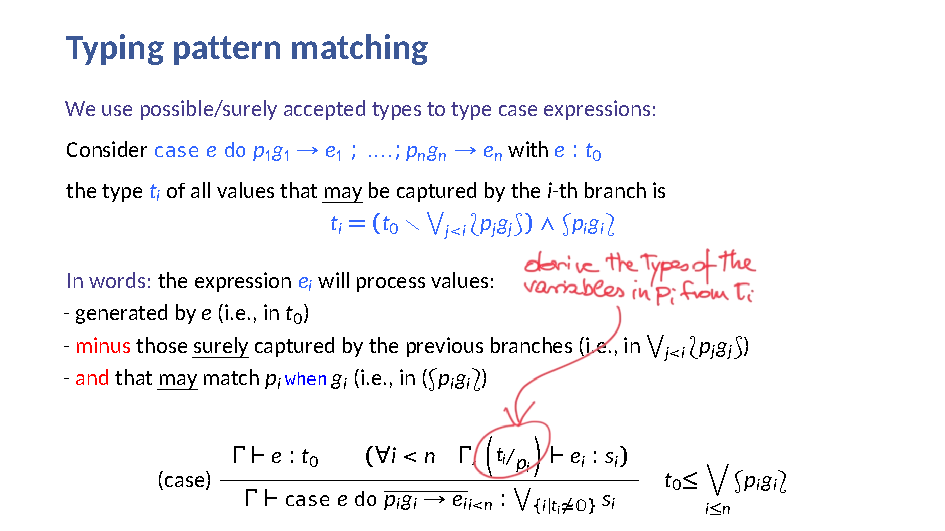
\includegraphics[scale=1]{images/slide-caserule1.pdf}
\end{textblock}}
\only<9>{\begin{textblock}{5}(0,0)
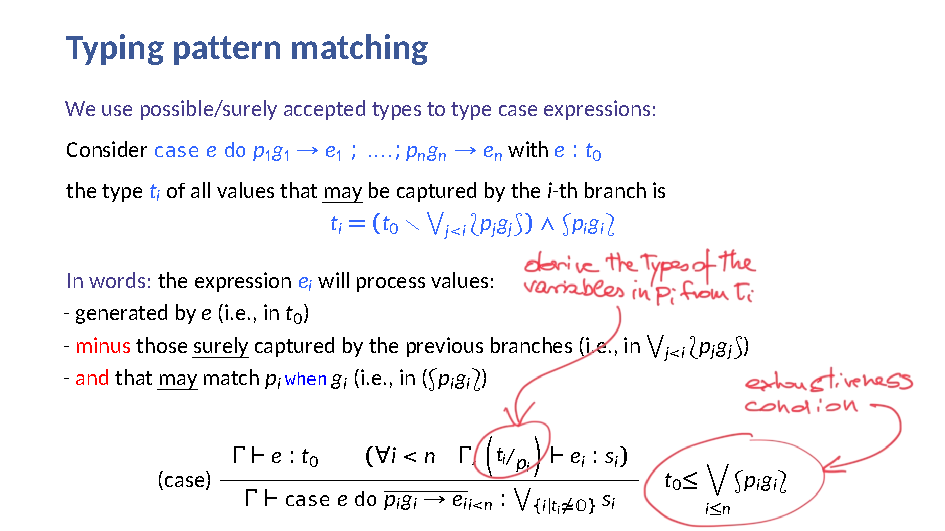
\includegraphics[scale=1]{images/slide-caserule2.pdf}
\end{textblock}}
\only<10>{\begin{textblock}{5}(0,0)
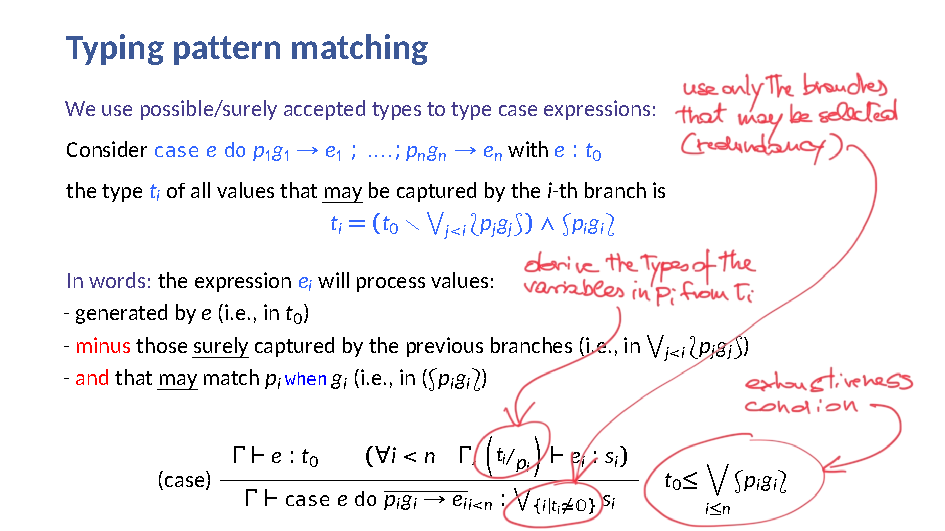
\includegraphics[scale=1]{images/slide-caserule3.pdf}
\end{textblock}}
\end{frame}



\begin{frame}[fragile]
\frametitle{Precise Guard Analysis}

\textbf{\color{darkslateblue}For each pattern guard we deduce a \emph{list} of flagged types (by decomposing the guard in OR-clauses):}
\vspace{-2mm}
\[\Gamma\vdash p_ig_i \leadsto [(s_{ij},\BoolB_{ij})]_{j\leq m_i}\]


%\only<2>{\vspace{-1.7mm}}

\

% \pause\pause
% \only<3>{\begin{textblock}{5}(0,0)
% \includegraphics[scale=1]{images/guardanalysis1.pdf}
% \end{textblock}}
% \only<4>{\begin{textblock}{5}(0,0)
% \includegraphics[scale=1]{images/guardanalysis2.pdf}
% \end{textblock}}

\pause\pause
\pause 
\begin{block}{Guard Analysis}
Consider again \quad $pg$ \quad =\quad   {\color{typeGreen}\code{x when (is_map(x) and map_size(x) == 2) or
  is_list(x)}}
\pause
   $\Gamma,\texttt{term()}\vdash [ pg ] \leadsto$ [(\code{map()},\code{false}),
      (\code{list()},\code{true})]

\pause
    $\sAccType{pg}\quad=\quad$  {\color{typeGreen}\code{list()}}\hfill (all types in the list with
\code{true} flag)\vspace{-1mm}

    $\pAccType{pg}\quad=\quad$   {\color{typeGreen}\code{map() or list()}} \hfill (all types in the
list with any flag)

\end{block}
\pause
\structure{\bf Fine-grained analysis needed to  infer the type of}
\begin{minted}{elixir}
def baz(x, y) when is_boolean(x) or is_integer(y), do: {y,x} 
#=> ((term(),integer()) -> {integer(),term()}) and
#   ((boolean(),term()) -> {term(),boolean()})
\end{minted}
\only<2>{\begin{textblock}{5}(0,0)
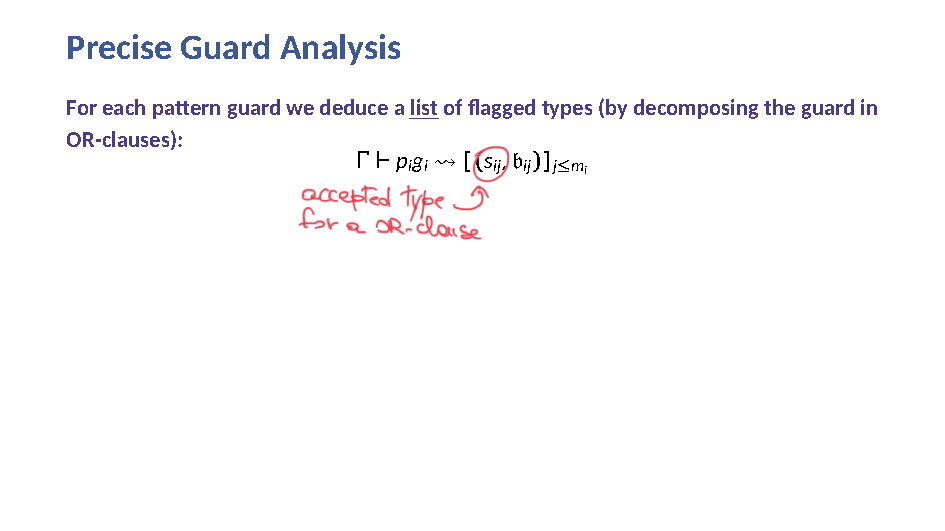
\includegraphics[scale=1]{images/slide-guardtype.pdf}
\end{textblock}}
\only<3>{\begin{textblock}{5}(0,0)
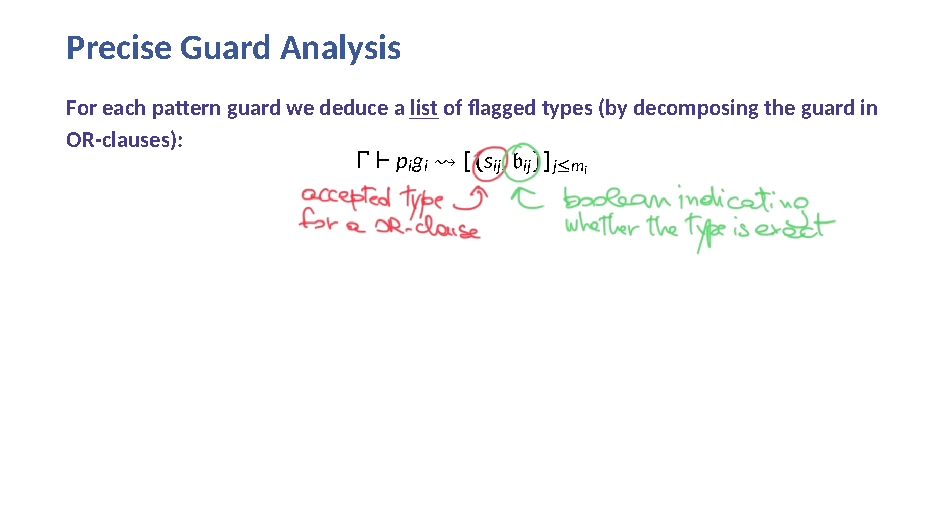
\includegraphics[scale=1]{images/slide-guardbool.pdf}
\end{textblock}}
\end{frame}
